\documentclass[a4paper,11pt]{article}
\usepackage[T1]{fontenc}
\usepackage{newtxtext,newtxmath}
\usepackage[margin=22mm]{geometry}
\usepackage{booktabs,tabularx,array,graphicx,tikz}
\usetikzlibrary{arrows.meta,calc,backgrounds}
\usepackage[font=small,labelfont=bf]{caption}
\usepackage[hidelinks]{hyperref}
\usepackage{xcolor}
\hypersetup{colorlinks=false,pdfborder={0 0 0},pdftitle={Cloud models and survey architecture},pdfauthor={Member 2}}
\color{black}
\linespread{1.05}
\setlength{\parskip}{3pt}
\setlength{\parindent}{1em}
\setlength{\textfloatsep}{12pt}
\setlength{\intextsep}{11pt}
\setlength{\tabcolsep}{7pt}
\renewcommand{\arraystretch}{1.13}
\renewcommand{\thetable}{\Roman{table}}
\makeatletter
\renewcommand\section{\@startsection{section}{1}{0pt}{11pt}{5pt}{\normalfont\large\bfseries}}
\makeatother
\newif\ifcountonly
\ifdefined\CountOnly\countonlytrue\else\countonlyfalse\fi
\begin{document}
\begin{center}{\large\bfseries Cloud models and survey architecture}\end{center}
\vspace{-6pt}
\section*{A-II Cloud models and actors}

Company A consumes Google's platform and provides SaaS to respondents; Table~\ref{tab:actors} distinguishes the actor roles~\cite{nist}. Direct contracting needs no broker. An independent auditor could assess either service; none is appointed.

\begin{table}[htbp]
\centering
\caption{Actors at the two service boundaries}
\label{tab:actors}
\ifcountonly\else
\begin{tabular}{@{}lcc@{}}
\toprule
Actor & Consumed platform & Provided survey \\
\midrule
Consumer & Company A & Respondents \\
Provider & Google & Company A \\
Carrier & Internet providers & Internet providers \\
Broker & None required & None required \\
Auditor & Independent assessor & Independent assessor \\
\bottomrule
\end{tabular}
\fi
\end{table}

Table~\ref{tab:responsibility} compares the same workload. Service models allocate operational work; deployment models determine access and infrastructure exclusivity. Combining service models is not hybrid cloud, and a public-cloud VPC alone is not a private cloud~\cite{nist}. SaaS requires checking ID lookup and exports.

\begin{table}[htbp]
\centering
\caption{Management responsibility for the survey workload}
\label{tab:responsibility}
\ifcountonly\else
\small
\begin{tabularx}{\linewidth}{@{}Xccc@{}}
\toprule
Responsibility & IaaS VM & \shortstack{PaaS/serverless\\(Cloud Run)} & SaaS survey \\
\midrule
Physical infrastructure & Vendor & Vendor & Vendor \\
Guest/host operating system & Company A & Vendor & Vendor \\
Image/runtime dependencies & Company A & Company A & Vendor \\
Application & Company A & Company A & Vendor \\
Data/access policies & Company A & Company A & Company A \\
Scaling rules & Company A & Company A & Vendor \\
Scaling execution & Company A & Vendor & Vendor \\
\bottomrule
\end{tabularx}
\fi
\end{table}

Cloud Run manages execution; Company A maintains its image and dependencies~\cite{container}. A managed-runtime PaaS would move runtime maintenance to the vendor.

XMDrive is SaaS: XMUM documents campus-ID login, off-campus browser access and a 5~GB student allocation~\cite{xmdrive}. Institutional membership supports a provisional private-cloud classification, although exclusive infrastructure is unconfirmed. Broad network access and file-upload self-service are visible, but uploading is not infrastructure provisioning. Quotas suggest storage measurement without proving billing transparency. Resource pooling is undisclosed, while fixed allocations give students little evidence of rapid elasticity.


\section*{B-II Architecture and design justification}

Figure~\ref{fig:architecture} places Google Cloud Run in Singapore. The service model is serverless PaaS; the deployment model is public cloud. This removes VM host-OS maintenance and scaling execution. Private infrastructure would add hardware and control-plane administration for three IT staff. The proposed managed features are generally available; documentation was checked on 18~November~2026.

\begin{figure}[tbp]
\centering
\resizebox{\linewidth}{!}{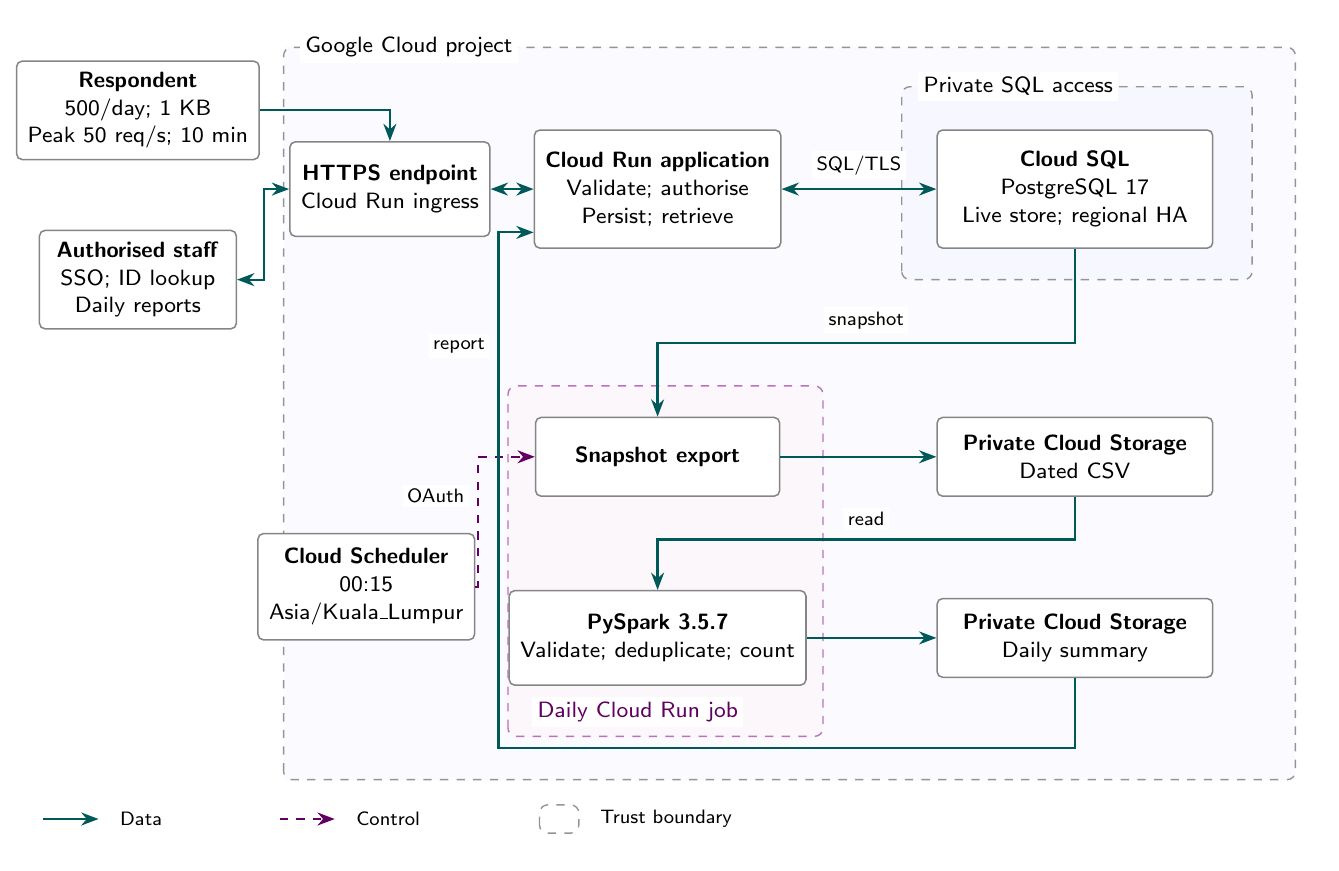
\begin{tikzpicture}[x=1cm,y=1cm,
font=\sffamily\fontsize{8.3}{10}\selectfont,
box/.style={draw=black!48,fill=white,rounded corners=2pt,align=center,inner sep=4pt,line width=.55pt},
data/.style={-{Stealth[length=2.2mm]},draw=teal!70!black,line width=.8pt},
both/.style={arrows={Stealth[length=2.2mm]-Stealth[length=2.2mm]},draw=teal!70!black,line width=.8pt},
control/.style={-{Stealth[length=2.2mm]},draw=violet!75!black,dashed,line width=.8pt},
flowlabel/.style={font=\sffamily\fontsize{7.5}{9}\selectfont,fill=white,inner sep=1.6pt,text=black},
boundary/.style={draw=black!42,dashed,rounded corners=3pt,line width=.5pt},
title/.style={font=\sffamily\fontsize{8}{9.5}\selectfont,text=black,fill=white,inner sep=2pt}]
% Labels stay in fixed boxes; flow labels have an explicit gap from the route.
% x=5.98 is reserved for the report-return corridor.
\path[use as bounding box] (0,-.8) rectangle (16.3,9.55);
\begin{scope}[on background layer]
\fill[blue!2] (3.25,0) rectangle (16.1,9.3);
\draw[boundary] (3.25,0) rectangle (16.1,9.3);
\draw[boundary,fill=blue!3] (11.1,6.35) rectangle (15.55,8.8);
\draw[boundary,draw=violet!55,fill=violet!3] (6.1,.55) rectangle (10.1,5.0);
\end{scope}
\node[title,anchor=west] at (3.45,9.3) {Google Cloud project};
\node[title,anchor=west] at (11.3,8.8) {Private SQL access};
\node[title,anchor=west,text=violet!75!black] at (6.4,.86) {Daily Cloud Run job};
\node[box,minimum width=2.5cm,minimum height=1.25cm] (respondent) at (1.4,8.5)
{\textbf{Respondent}\\500/day; 1 KB\\Peak 50 req/s; 10 min};
\node[box,minimum width=2.5cm,minimum height=1.25cm] (staff) at (1.4,6.35)
{\textbf{Authorised staff}\\SSO; ID lookup\\Daily reports};
\node[box,minimum width=2.1cm,minimum height=1.2cm] (endpoint) at (4.6,7.5)
{\textbf{HTTPS endpoint}\\Cloud Run ingress};
\node[box,minimum width=3cm,minimum height=1.5cm] (app) at (8,7.5)
{\textbf{Cloud Run application}\\Validate; authorise\\Persist; retrieve};
\node[box,minimum width=3.5cm,minimum height=1.5cm] (sql) at (13.3,7.5)
{\textbf{Cloud SQL}\\PostgreSQL 17\\Live store; regional HA};
\node[box,minimum width=2.5cm,minimum height=1.35cm] (scheduler) at (4.3,2.45)
{\textbf{Cloud Scheduler}\\00:15\\Asia/Kuala\_Lumpur};
\node[box,minimum width=3.1cm,minimum height=1cm] (export) at (8,4.1)
{\textbf{Snapshot export}};
\node[box,minimum width=3.1cm,minimum height=1.2cm] (spark) at (8,1.8)
{\textbf{PySpark 3.5.7}\\Validate; deduplicate; count};
\node[box,minimum width=3.5cm,minimum height=1cm] (csv) at (13.3,4.1)
{\textbf{Private Cloud Storage}\\Dated CSV};
\node[box,minimum width=3.5cm,minimum height=1cm] (summary) at (13.3,1.8)
{\textbf{Private Cloud Storage}\\Daily summary};
\draw[data] (respondent.east) -- (4.6,8.5) -- (endpoint.north);
\draw[both] (staff.east) -- (3.0,6.35) -- (3.0,7.5) -- (endpoint.west);
\draw[both] (endpoint.east) -- (app.west);
\draw[both] (app.east) -- node[flowlabel,above=3pt] {SQL/TLS} (sql.west);
\draw[data] (sql.south) -- (13.3,5.55) --
node[flowlabel,above=3pt] {snapshot} (8,5.55) -- (export.north);
\draw[control] (scheduler.east) -- (5.72,2.45) --
node[flowlabel,left=3pt,pos=.7] {OAuth} (5.72,4.1) -- (export.west);
\draw[data] (export.east) -- (csv.west);
\draw[data] (csv.south) -- (13.3,3.05) --
node[flowlabel,above=3pt] {read} (8,3.05) -- (spark.north);
\draw[data] (spark.east) -- (summary.west);
\draw[data] (summary.south) -- (13.3,.4) -- (5.98,.4) --
node[flowlabel,left=3pt,pos=.78] {report} (5.98,6.95) -- ($(app.west)+(0,-.55)$);
\draw[data] (.2,-.5) -- (.9,-.5);
\node[anchor=west,font=\sffamily\fontsize{7.5}{9}\selectfont] at (1.05,-.5) {Data};
\draw[control] (3.2,-.5) -- (3.9,-.5);
\node[anchor=west,font=\sffamily\fontsize{7.5}{9}\selectfont] at (4.05,-.5) {Control};
\draw[boundary] (6.5,-.68) rectangle (7,-.32);
\node[anchor=west,font=\sffamily\fontsize{7.5}{9}\selectfont] at (7.15,-.5) {Trust boundary};
\end{tikzpicture}

}
\caption{Proposed survey architecture in \texttt{asia-southeast1}. Solid arrows carry data; dashed arrows invoke jobs. Dashed enclosures mark trust or service-identity boundaries.}
\label{fig:architecture}
\end{figure}

HTTPS submissions accept only Good, OK or Poor. Valid responses enter Cloud SQL PostgreSQL~17, indexed by \texttt{response\_id}; support staff retrieve individual records through authenticated application routes. Direct VPC egress and TLS protect the database connection~\cite{connection}. Staff SSO and server-side roles restrict lookup and reporting; knowing an ID grants no permission.

At 00:15 Malaysia time, Cloud Scheduler invokes a Cloud Run job using OAuth~\cite{schedule}. It exports the previous day's consistent SQL snapshot to private Cloud Storage, then PySpark~3.5.7 validates ratings, deduplicates IDs and counts categories locally~\cite{storage,spark}. SQL supplies Bigtable-like serving, dated files fulfil GFS-like storage, and aggregation follows MapReduce's processing role~\cite{bigtable,gfs,mapreduce}. These are role comparisons, not identical mechanisms. Daily results return through the staff application; Cloud Storage replaces manual XMDrive sharing.

Stateless instances expand during the ten-minute campaign and return to zero afterwards, accepting cold starts~\cite{scaling}. Assuming 0.5~s per request, 50~requests/s require 25 concurrent requests; four instances at concurrency~20 leave headroom. This assumption needs validation. Limiting each instance to five database connections controls connection growth. Monitor latency, errors and instance count; temporary instance overshoot and alerts-only budgets prevent a hard spending guarantee~\cite{scaling,budgets}. SQL remains billable while the application is idle.

An instance failure preserves committed database rows; idempotent retries recover interrupted requests. Regional SQL high availability addresses zonal failure, while backups and point-in-time recovery address deletion~\cite{ha}. These do not provide cross-region disaster recovery.

Use separate service identities, least privilege, encryption at rest, consent/notices, log redaction and correction access. Delete records and retained copies after the case's three-year period. Singapore processing requires documented PDPA transfer grounds~\cite{pdpa,transfer}.

An OpenStack~2025.2 private cloud could use Nova VMs, Neutron networks, Cinder database volumes, Swift exports and Keystone identities~\cite{openstack}. Company A would then own hardware, patching, capacity, database failover and backups. Exclusivity does not justify that operating burden unless it becomes a firm requirement.


\ifcountonly\else\begin{thebibliography}{99}
\setlength{\itemsep}{1.5pt}\small
\bibitem{nist}
F. Liu \emph{et al.}, \href{https://www.nist.gov/publications/nist-cloud-computing-reference-architecture}{\emph{NIST Cloud Computing Reference Architecture}}, NIST SP~500-292, 2011.
\bibitem{container}
Google Cloud, \href{https://docs.cloud.google.com/run/docs/container-contract}{\emph{Container runtime contract}}. Accessed: Nov.~18, 2026.
\bibitem{xmdrive}
XMUM LINC, \href{https://linc.xmu.edu.my/online-storage/}{\emph{Online Storage}}. Accessed: Nov.~18, 2026.
\bibitem{connection}
Google Cloud, \href{https://docs.cloud.google.com/sql/docs/postgres/connect-run}{\emph{Connect from Cloud Run}}. Accessed: Nov.~18, 2026.
\bibitem{schedule}
Google Cloud, \href{https://docs.cloud.google.com/run/docs/execute/jobs-on-schedule}{\emph{Execute jobs on a schedule}}. Accessed: Nov.~18, 2026.
\bibitem{storage}
Google Cloud, \href{https://docs.cloud.google.com/storage/docs/public-access-prevention}{\emph{Public access prevention}}. Accessed: Nov.~18, 2026.
\bibitem{spark}
Apache Spark, \href{https://spark.apache.org/releases/spark-release-3-5-7.html}{\emph{Spark Release 3.5.7}}, 2025.
\bibitem{bigtable}
F. Chang \emph{et al.}, \href{https://research.google/pubs/bigtable-a-distributed-storage-system-for-structured-data/}{\emph{Bigtable: A distributed storage system for structured data}}, in OSDI, 2006, pp.~205--218.
\bibitem{gfs}
S. Ghemawat, H. Gobioff, and S.-T. Leung, \href{https://research.google/pubs/the-google-file-system/}{\emph{The Google File System}}, in SOSP, 2003, pp.~29--43.
\bibitem{mapreduce}
J. Dean and S. Ghemawat, \href{https://research.google/pubs/mapreduce-simplified-data-processing-on-large-clusters/}{\emph{MapReduce: Simplified data processing on large clusters}}, in OSDI, 2004, pp.~137--150.
\bibitem{scaling}
Google Cloud, \href{https://docs.cloud.google.com/run/docs/about-instance-autoscaling}{\emph{About instance autoscaling in Cloud Run services}}. Accessed: Nov.~18, 2026.
\bibitem{budgets}
Google Cloud, \href{https://docs.cloud.google.com/billing/docs/how-to/budgets}{\emph{Create, edit, or delete budgets and budget alerts}}. Accessed: Nov.~18, 2026.
\bibitem{ha}
Google Cloud, \href{https://docs.cloud.google.com/sql/docs/postgres/high-availability}{\emph{About high availability}}. Accessed: Nov.~18, 2026.
\bibitem{pdpa}
Personal Data Protection Department, \href{https://www.pdp.gov.my/en/principles-of-personal-data-protection/}{\emph{Principles of Personal Data Protection}}. Accessed: Nov.~18, 2026.
\bibitem{transfer}
Personal Data Protection Department, \href{https://www.pdp.gov.my/ppdpv1/wp-content/uploads/2025/08/GP_CBPDT_EN.pdf}{\emph{Cross Border Personal Data Transfer}}, Guideline~3/2025, 2025.
\bibitem{openstack}
OpenStack, \href{https://releases.openstack.org/flamingo/}{\emph{2025.2 Flamingo}}. Accessed: Nov.~18, 2026.
\end{thebibliography}

\fi
\end{document}

